\documentclass[serif,compress, blue, 11pt]{beamer}
\mode<presentation>
\usetheme{Berlin}
\useoutertheme[subsection=false]{smoothbars}

% include packages
\usepackage{subfigure}
\usepackage{multicol}
\usepackage{amsmath}
\usepackage{epsfig}
\usepackage{graphicx}
\usepackage[all,knot]{xy}
\xyoption{arc}
\usepackage{url}
\usepackage{multimedia}
\usepackage{hyperref}
\usepackage{setspace}
\graphicspath{{/home/corwin/Documents/ipm/publication/abstracts/2017}}

\setbeamerfont{frametitle}{size=\small}

% Seven International Scientific School for Young Scientists "Waves and vortices in complex media".

\title[Waves and vortices in complex media]{\textbf{Singularity and limiting cases for oscillations in a viscous
continuously stratified fluid problems}}
\author[Alexey Vasiliev]{%
  Alexey~Vasiliev}
\institute[Institute for Problems in Mechanics of the RAS]{Laboratory of Fluid Mechanics\\
  Institute for Problems in Mechanics of the RAS\\
  Moscow, Russia
  }
\date[2017]{Seven International Scientific School for Young Scientists "Waves and vortices in complex media".}

\begin{document}

\frame{
	\titlepage
}

\section{Intro}


\subsection{Color schlirien images oscillation of disk}
\frame{\frametitle{Color shadow image of disk oscillation.}
\begin{figure}
\center 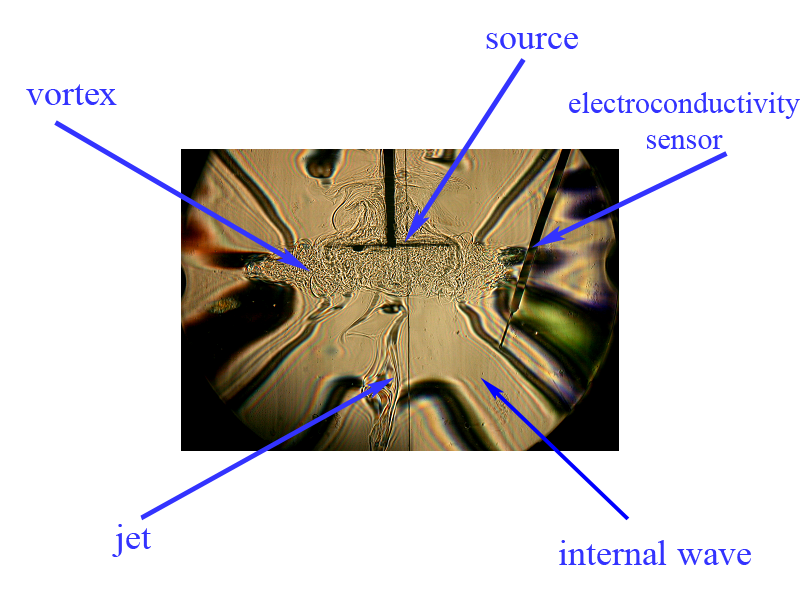
\includegraphics[width=0.98\linewidth]{disk2-descr.png} 
\end{figure}}

\subsection{Formulation of the problem.}
\frame{\frametitle{Formulation of the problem.}
\begin{figure}
   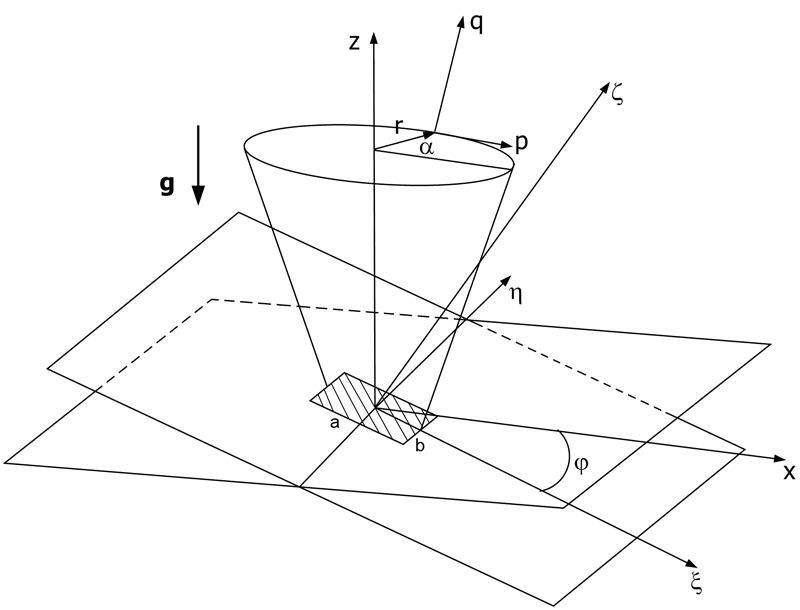
\includegraphics[width=0.8\linewidth]{sys-coord.png}
\end{figure}
}

\section{General solutions}
\subsection{Governing equations and boundary conditions}
\frame{\frametitle{Governing equations and boundary conditions.}
\textbf{Governing equations}
\[
\frac{{\partial \rho} }{{\partial t}} + \textbf{v} \nabla \rho = 0,
\quad
\operatorname{div}\; \textbf{v} = 0
\]
\[
\frac{{\partial \textbf {v}} }{{\partial t}} + \left( {\textbf{v},\nabla} \right) \textbf{v} = \frac{1}{\rho} \nabla p + \nu \Delta v + \rho \textbf{g}
\]
\[
\frac{{\partial S} }{{\partial t}} = \kappa_S \Delta S + \frac{v_z}{\Lambda} 
\]
\textbf{Boundary conditions}
\[
\left. {\textbf{v}} \right|_{\Gamma}  = \textbf{u}_{0} e^{ - i\omega t},
\quad
\kappa _{S} \left. {\frac{{\partial S}}{{\partial n}}} \right|_{\Gamma}  = 0
\]

%Infinity conditions
\[
 v \to 0,
\quad
\rho \to \rho _{0} ,
\quad
{{\partial P} \mathord{\left/ {\vphantom {{\partial P} {\partial z}}} 
\right. \kern-\nulldelimiterspace} {\partial z}} \to \rho _{0} \left( {z} 
\right)g, r \to \infty
\]


\textbf{Toroidal-poloidar decomposition}
\[
\textbf{v} = 
\nabla \times \textbf{e}_{z} \Phi + \nabla \times \left( {\nabla \times \textbf{e}_{z} \Psi}  
\right)
\]

}

\frame{\frametitle{System equation for scalar function $\Phi$ and $\Psi$}
\[
\left( {\left( {\frac{{\partial} }{{\partial t}} - D\Delta}  \right)\left( 
{\frac{{\partial} }{{\partial t}} - \nu \Delta}  \right)\Delta + N^{2}\Delta 
_{ \bot} }  \right)\;\Phi = 0
\]

\[
\left( {\frac{{\partial} }{{\partial t}} - 
\nu \Delta}  \right)\;\Psi = 0
\]

\[
\left( {\left( {\frac{{\partial} }{{\partial t}} - D\Delta}  \right)\left( 
{\frac{{\partial} }{{\partial t}} - \nu \Delta}  \right)\Delta + N^{2}\Delta 
_{ \bot} }  \right)\;S = 0
\]

where 
\[
\Delta _{ \bot}  = \partial _{x} ^{2} + \partial _{y} ^{2} 
\quad
\Delta  = \partial _{x} ^{2} + \partial _{y} ^{2} +\partial_{z}^2
\quad
N^2=\sqrt{\frac{g}{\Lambda}}
\]
}

\section{Analysis of the solution}
\subsection{Dispersion equation}

\frame{\frametitle{The viscous stratified fluid taking into account effects of diffusion}
\textbf{Dispersion equation}
\[
\left( {\nu \kappa _{S} \tilde {k}^{6} - i\omega \left( {\nu + \kappa _{S}}  
\right)\tilde {k}^{4} - \omega ^{2}\tilde {k}^{2} + N^{2}k_{ \bot} ^{2}}  
\right) \left( \tilde{k}^{2} + \frac{\omega}{i\nu} \right) = 0
\]

\[
\tilde {k}^{2} = 2k_{\zeta} ^{2} + k_{ \bot} ^{2} ,
\quad
k_{ \bot} ^{2} = k_{\xi} ^{2} + k_{\eta} ^{2} 
\]

\textbf{Regular solution}
\[
 k_{1} = \frac{{k_{\xi}  \sin\varphi \cos\varphi \pm \kappa \cos\theta} }{{\mu_{\theta}} } 
\pm \delta _{N}^{2} \left( {1 + \varepsilon}  \right)\frac{{i\; \tan\theta \mu_{\theta}^{4}}}{{2\kappa \mu 
^{4}}} + ...
\]

\[
\mu = \sin^{2}\varphi - \sin^{2}\theta,
\quad
\mu_{\theta} = \left({k_{\xi}  \sin\varphi \cos\varphi \pm \kappa \cos\varphi}  \right),
\]
\[
 \varepsilon = Sc^{ - 1} = \frac{{\kappa _{S}} }{{\nu} },
\quad
 \delta _{N} = \sqrt {\frac{{\nu} }{{N}}} 
\]

}

\frame{\frametitle{The viscous stratified fluid taking into account effects of diffusion}
\textbf{Singular solutions} \\
\[
k_{2,\;3} \approx \sqrt {\frac{{i\omega \left( {\varepsilon + 1 \pm \lambda 
_{\nu \kappa} }  \right)}}{{\varepsilon} }} ,
\quad
\lambda _{\nu \kappa}  = \frac{{2}}{{\sin\theta} }\sqrt {\left( {1 + 
\varepsilon}  \right)^{2} - \frac{{4\varepsilon \mu} }{{\sin^{2}\theta} }}
\]

\vspace{0.25cm}

\[
 k_{4} = \sqrt {\frac{{2i}}{{\delta _{\nu} ^{2}} } - k^{2}},
\quad
\delta _{\nu}  = \delta _{N} \sqrt {\frac{{2}}{{\sin\theta} }} 
\]
}

\subsection{General solution}
\frame{\frametitle{The viscous stratified fluid taking into account effects of diffusion}

\[
v_{\xi}  \approx - \frac{{1 - i}}{{2}}\delta _{\varphi}  G_{1} + \frac{{i\delta 
_{N}^{2}} }{{\sqrt {\left| {\mu}  \right|}} }\tan^{2}\varphi \,\,G_{2} - G_{3} ,
\]

\[
 Q_n = u_0 \int\limits_{ - \infty} ^{ + \infty}
 \frac{g_n}{k^2_{\eta}\cos\varphi + k_{\xi}\beta} \, dk_{\xi}  dk_{\eta} ,
 \quad
 \beta = k_{\xi}\cos\varphi - k_1\sin\varphi,
\]

\[
 g_0 = \gamma k_{\xi} k_{\eta} e_1,
 \quad
 g_1 = k_{\xi}e_1\left(k^2_{\eta}\sin\varphi-k_1\beta\right),
\]

\[
 g_2 = k_{\eta}Q\exp\left(\frac{i-1}{\delta_{\nu}\xi}\right)\left[k^2_{\eta}\cos\varphi + k_{\xi}\left(k_1-\gamma\right)\right] ,
 \quad
 Q = e^{i\left(k_{\xi}\xi+k_{\eta}\eta\right)},
\]

\[
 g_3 = k_{\eta}Q\exp\left(-\frac{i+1}{\delta_{\nu}\xi}\right)\left(k^2_{\eta}\sin\varphi + k_{\xi}\beta\sin\varphi\right),
 \quad
 \gamma = k_{\xi}\sin\varphi + k_1\cos\varphi
\]

}

\frame{\frametitle{The viscous stratified fluid taking into account effects of diffusion}
\[
v_{\eta}  \approx \left( {1 - i} \right)\delta _{\varphi}  G_{0} + \frac{{1 - 
i}}{{2}}\delta _{\nu}  \tan\varphi \,G_{2} - \left( {1 - i} \right)\delta _{\varphi 
} \frac{{\cos\varphi} }{{\sin^{2}\varphi} }G_{3} 
\]

\[
v_{\zeta}  \approx \frac{{i - 1}}{{2}}\delta _{\varphi}  \int\limits_{ - \infty 
}^{ + \infty}  {u_{0} k_{\xi} }  e_{1} \,dk_{\xi}  dk_{\eta}  + 
\frac{{i\delta _{N}^{2}} }{{2\sqrt {\left| {\mu}  \right|}} }\tan\varphi \,G_{2} 
- \frac{{1 + i}}{{\delta _{\varphi}  \sin\varphi} }G_{3} 
\]
}



\section{limiting cases}
\subsection{phi=0}

\frame{\frametitle{The viscous stratified fluid. Friction source. Rectangle. 3D. $\varphi = 0$.}
\[
v_{\xi}  = \int\limits_{ - \infty} ^{ + \infty}  {k_{\eta} ^{2} L_{3} \,} 
dk_{\xi}  dk_{\eta}  + \int\limits_{ - \infty} ^{ + \infty}  {k_{\xi} ^{2} 
L_{1}}  \,dk_{\xi}  dk_{\eta}  ,
\]

\[
v_{\eta}  = \int\limits_{ - \infty} ^{ + \infty}  {L_{3}}  \,dk_{\xi}  
dk_{\eta}  + \int\limits_{ - \infty} ^{ + \infty}  {k_{\xi}  k_{\eta}  L_{1} 
} \,dk_{\xi}  dk_{\eta}, 
\quad
v_{\zeta}  = \int\limits_{ - \infty} ^{ + \infty}  {k_{\eta}  k_{ \bot} ^{2} 
} {\kern 1pt} L_{2} {\kern 1pt} dk_{\xi}  dk_{\eta}  
\]

\[
L_{m} = u_{0} Q\frac{{k_{1}^{2 - m} \exp\left( {ik_{1} \zeta}  \right) + 
k_{2}^{2 - m} \exp\left( {ik_{2} \zeta}  \right)}}{{\left( {k_{\eta} ^{2} - 
k_{\xi} ^{2}}  \right)\left( {k_{2} - k_{1}}  \right)}},
\quad
m = 1,2,
\]

\[
L_{3} = \frac{{u_{0} Q}}{{k_{\eta} ^{2} - k_{\xi} ^{2}} }\exp\left( { - 
\frac{{1 - i}}{{\delta _{\nu} } }\zeta}  \right)
\]
}

\subsection{2D case}
\frame{\frametitle{The viscous stratified fluid. Friction source. Plate. 2D.}

\[
v_{\xi}  = \frac{{u_{0}} }{{\pi ^{2}}}\int\limits_{ - \infty} ^{ + \infty}  
{\frac{{1}}{{k_{\xi}  \left( {k_{1} - k_{2}}  \right)}}\sin\frac{{k_{\xi}  
a}}{{2}}} \left( {k_{1} e^{ik_{1} \zeta}  - k_{2} e^{ik_{2} \zeta} } 
\right)e^{ik_{\xi}  \xi} dk_{\xi},
\]

\[
v_{\eta}  = 0,
\]

\[
v_{\zeta}  = \frac{{u_{0}} }{{\pi ^{2}}}\int\limits_{ - \infty} ^{ + \infty 
} {\frac{{1}}{{k_{2} - k_{1}} }\sin\frac{{k_{\xi}  a}}{{2}}} \left( 
{e^{ik_{1} \zeta}  + e^{ik_{2} \zeta} } \right)e^{ik_{\xi}  \xi} dk_{\xi},
\]

\[
k_{1} = k_{\xi}  \cot\left( {\varphi + \theta}\right)  \pm \frac{{ik_{\xi}  ^{3}\delta _{N}^{2} 
}}{{2\cos\theta \sin^{4}\left( {\varphi - \theta} \right) }},
\quad
k_{2} = \frac{{1 + i}}{{\delta _{\varphi} } }
\]

}

\subsection{Homogeneous fluid}

\frame{\frametitle{Homogeneous fluid $N\rightarrow0$}

\textbf{Solutions of the dispersion equation}

\[
k_{1} = k_{\bot}  
\quad
k_{2} = \frac{{1 + i}}{{\delta _{\varphi} } }
\quad
k_3 = \frac{1+i}{\delta_{\kappa}}
\quad
k_4 = k_2
\]

\[
 M_j = a_j\exp\left(-\sigma_{\kappa}\xi+i\frac{\zeta}{\sqrt{2}\delta_{\kappa}}\right)\sin^2\varphi
 \int\limits_{ - \infty} ^{ + \infty}A_3Qb_jdk_{\xi}dk_{\eta}
\]

\[
 \sigma_{\kappa} = \frac{\delta_N}{\delta_{\nu}\delta_{\kappa}}
\]



}

\frame{\frametitle{Homogeneous fluid $N\rightarrow$}

\textbf{Velocity components}

\[
\begin{array}{l}
v_{\xi}  = \int\limits_{ - \infty} ^{ + \infty}
A_1e_1\left(k_{\eta}^2\sin\varphi + k_1\beta_1\right)dk_{\xi}dk_{\eta}
\\
+ i\exp\left(-\frac{1-i}{\delta_{\nu}}\zeta \right) \int\limits_{ - \infty} ^{ + \infty}
\left(\frac{2}{\delta_{\nu}^2}+B\cos\varphi\right)Qdk_{\xi}dk_{\eta} + M_1
\end{array}
\]

\[
\begin{array}{l}
 v_{\eta} = \int\limits_{ - \infty} ^{ + \infty} 
 A_1\gamma_1e_1\kappa_1dk_{\xi}dk_{\eta}
 \\
 - \frac{1-i}{\delta_{\nu}}\exp\left(\frac{1-i}{\delta_{\nu}}\zeta\right)\int\limits_{ - \infty} ^{ + \infty}
 \left(A_2\kappa_{\eta}-B\sin\varphi\right)Qdk_{\xi}dk_{\eta} - M_2
 \\
\end{array}
\]

\[
 \begin{array}{l}
  v_{\zeta} = \int\limits_{ - \infty} ^{ + \infty} 
  A_1e_1\left(k_{\eta}^2\sin\varphi - k_{\eta}\beta\right)dk_{\xi}dk_{\eta}
  \\
  + i\exp\left(-\frac{1-i}{\delta_{\nu}}\zeta \right) \int\limits_{ - \infty} ^{ + \infty}
  \left(\frac{1-i}{\delta_{\varphi}} A_2k_{\xi} - B\sin\varphi\right) Q dk_{\xi}dk_{\eta} - M_3
 \end{array}
\]

}


\frame{\frametitle{Homogeneous fluid. Horizontal plane $N\rightarrow0$, $\varphi = 0$}
\[
 v_{\xi} = \int\limits_{ - \infty} ^{ + \infty}
 \left(k^2_{\eta}L_3dk_{\xi}dk_{\eta}+k^2_{\eta}L_1\right)dk_{\xi}dk_{\eta}
\]

\[
 v_{\eta} = \int\limits_{ - \infty} ^{ + \infty} 
 \left(L_3 + k_{\xi}k_{\eta}L_1\right)dk_{\xi}dk_{\eta}
\]

\[
 v_{\zeta} =  \int\limits_{ - \infty} ^{ + \infty}
 k_{\eta}k^2_{\bot}L_2dk_{\xi}dk_{\eta}
\]

\[
 L_m = u_0Q\frac{k^{2-m}_1e^{ik_1\zeta}+k^{2-m}_1e^{ik_2\zeta}}{(k^2_{\eta}-k^2_{\xi})(k_2-k_1)},
 \quad
 L_3 = \frac{u_0Q}{k^2_{\eta}-k^2_{\xi}}\exp\left(-\frac{1-i}{\delta_{\nu}}\zeta\right)
\]



}

\section{Comparisons}
\subsection{Displacement on the axis}
\frame{\frametitle{Displacement on the axis $h\left(0,q\right)$. Far field.}
%\rowcolors[]{1}{blue!20}{blue!10}
\begin{tabular}{|l|l|l|l|}
 \hline
 & & & \\
 Type of sources & Plane(2D) & Plane(3D) & Disk(3D)\\
 & & & \\
 \hline
 & & & \\
 Friction & $\frac{u_0}{N}\frac{a}{{\delta_N}^{1/3}}\frac{1}{q^{2/3}}$ & $\frac{u_0}{N}\frac{S}{\delta^{2/3}_N q^{4/3}}$ & $\frac{u_0}{\pi N}\frac{S}{{\delta_N}^{2/3}q^{4/3}}$\\
 & & & \\
 \hline
 & & & \\
 Piston & $\frac{u_0}{N}\frac{a}{{\delta_N}^{2/3}}\frac{1}{q^{1/3}}$ & $\frac{u_0}{N}\frac{S}{\delta_N q}$ & $\frac{u_0}{\pi N}\frac{S}{\delta_N q}$\\
 & & & \\
 \hline
 & & & \\
 Composite & $\frac{u_0}{N}\frac{a}{\delta^{4/3}_N}\frac{a}{q^{2/3}}$ & $\frac{u_0}{N}\frac{S}{\delta^{5/3}_N} \frac{b}{q^{4/3}}$ &  \\
 & & & \\
 \hline
\end{tabular}
}

\subsection{Comparison of the laboratory experiment (point) and calculations (lines) of the vertical displacement}
\frame{\frametitle{Comparison of the laboratory experiment (point) and calculations (lines) of the vertical displacement.}
\begin{figure}
   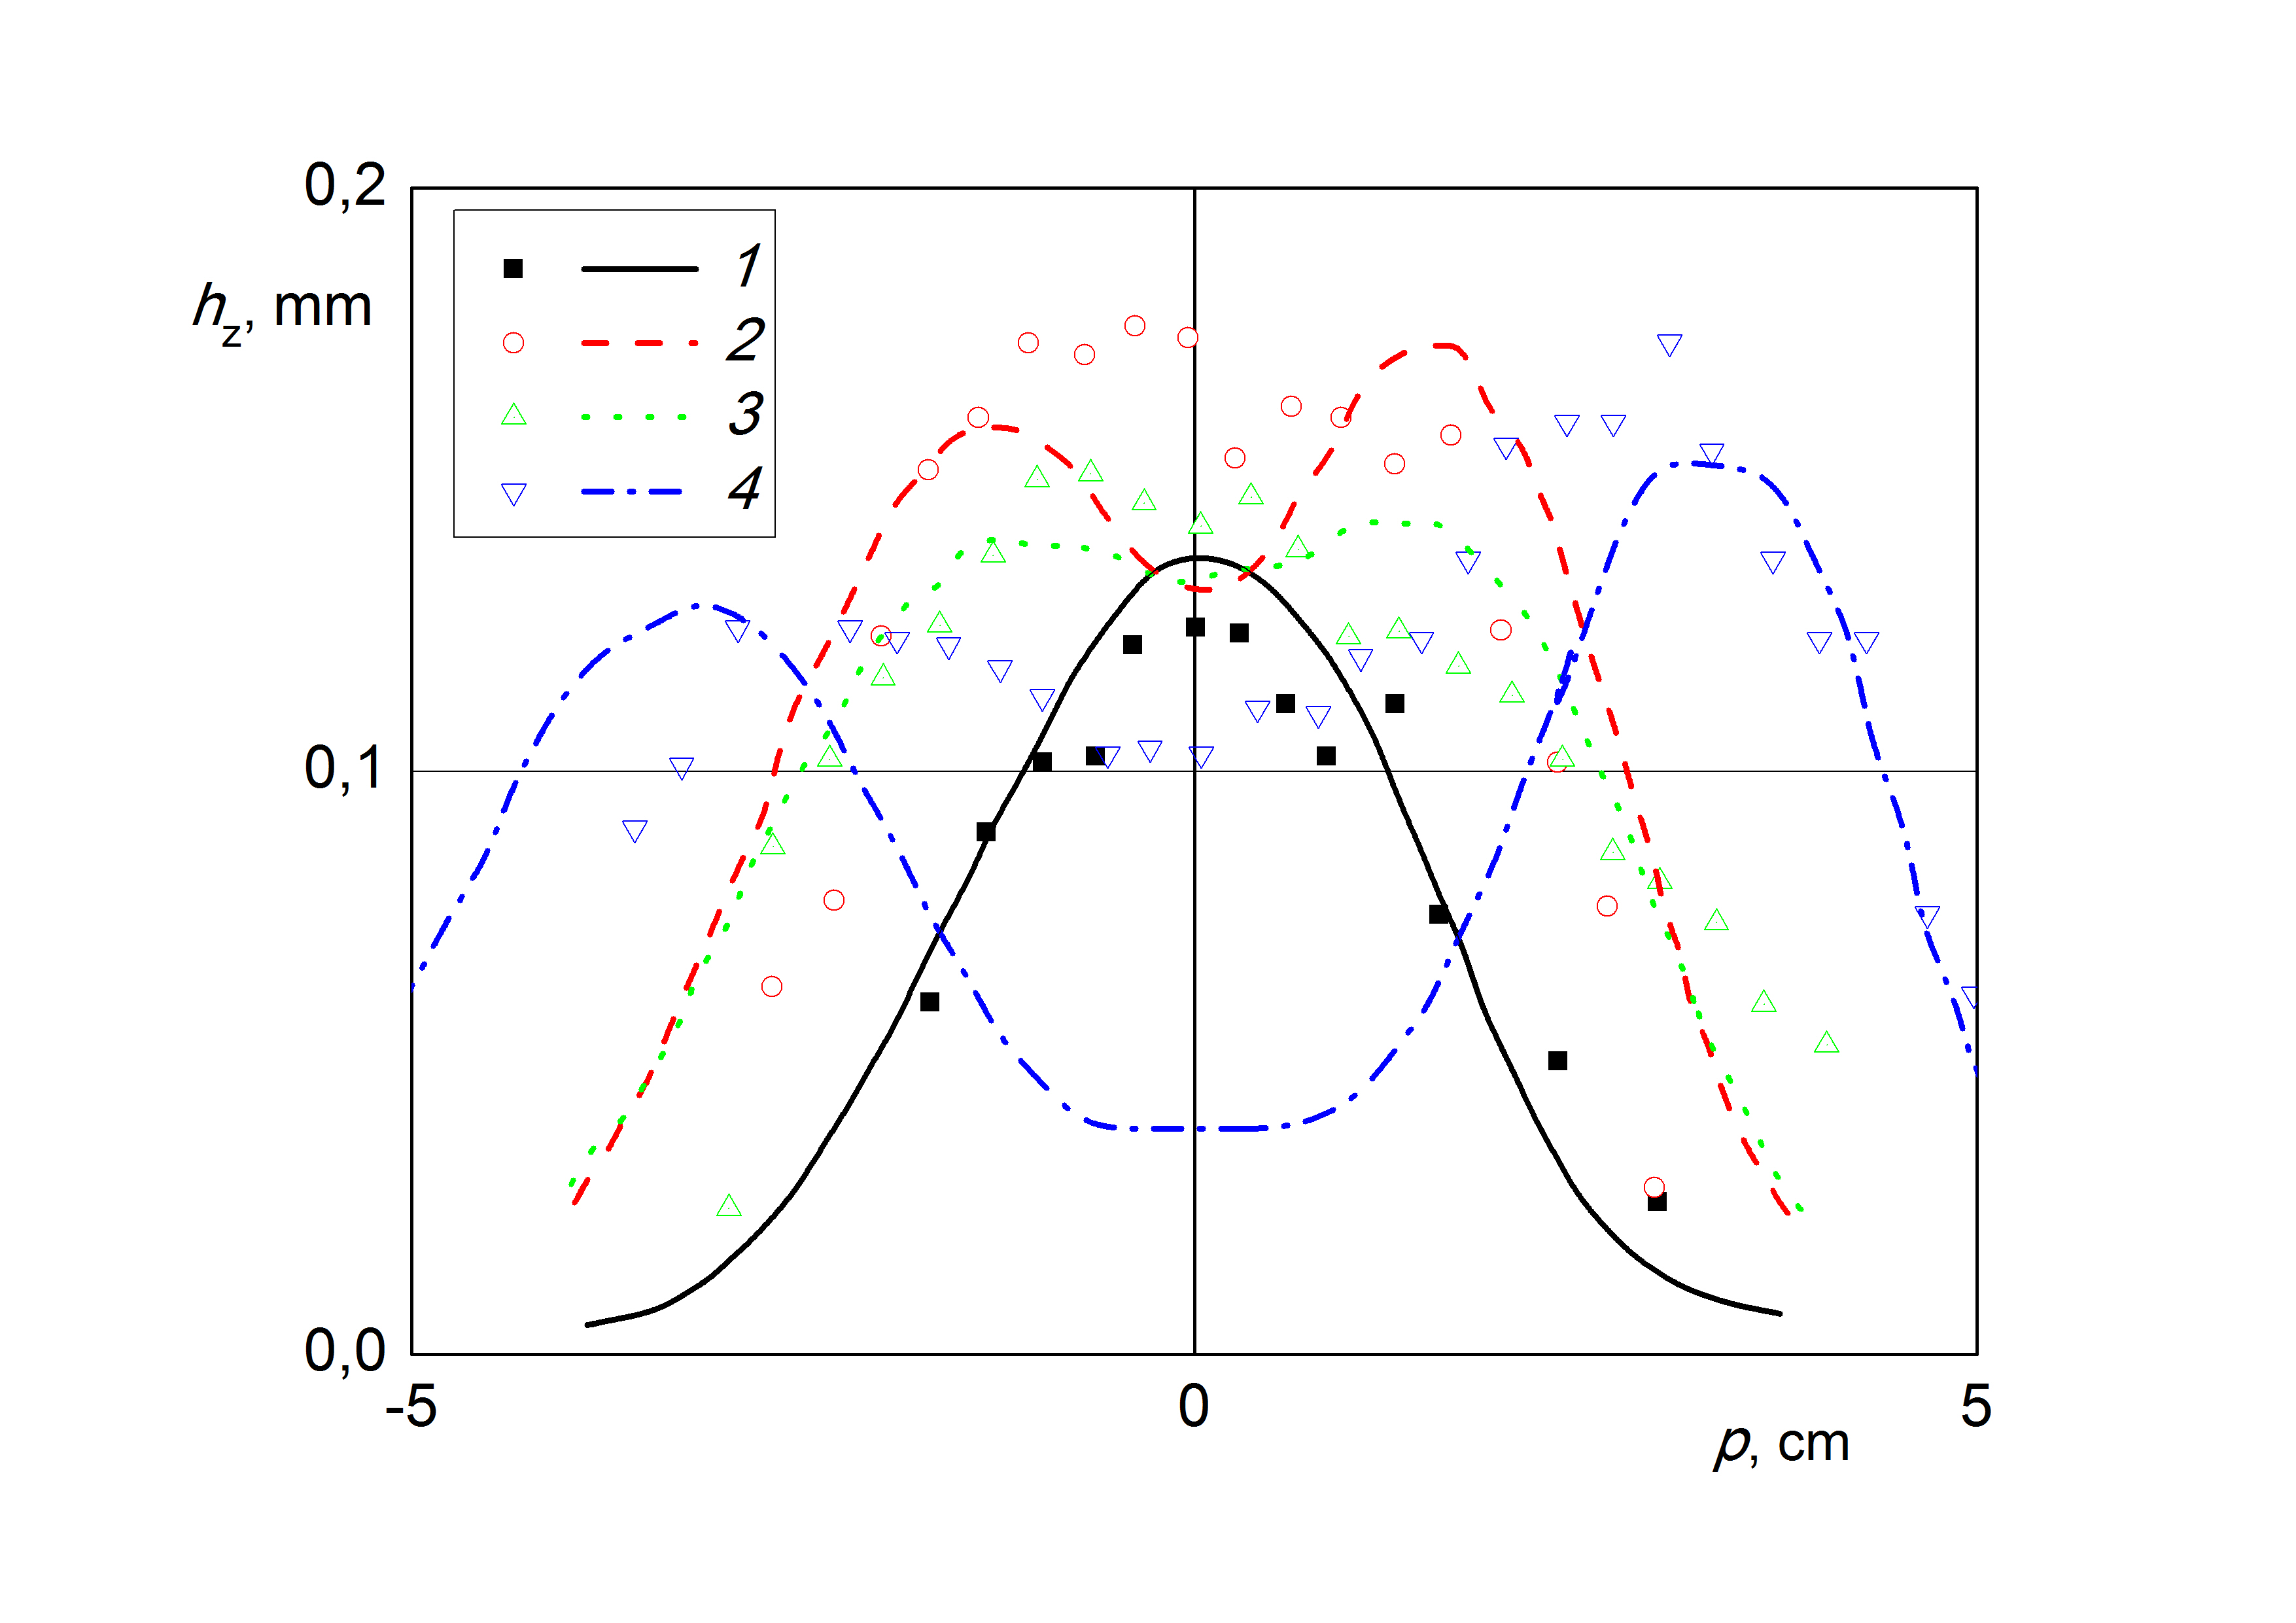
\includegraphics[width=0.8\linewidth]{compare.jpg}
\end{figure}
}

\section{Conclusions}
\frame{\frametitle{Conclusions:}
\begin{enumerate}
\item In general case there are the two type of flow: regular solution (internal waves) and three types of singular components of flow (boundary layers). 
Two of them have no analogue in a homogeneous fluid, their thickness is defined by dissipative factors;
\item Near the source viscosity and diffusion is basic factors;
\item The obtained results show that it is necessary to consider influence of dissipative factors (viscosity, stratification, diffusion).
\end{enumerate}
}

\end{document} 